% Describe the low-level communication protocols for all communications
\section{Communication Protocols}
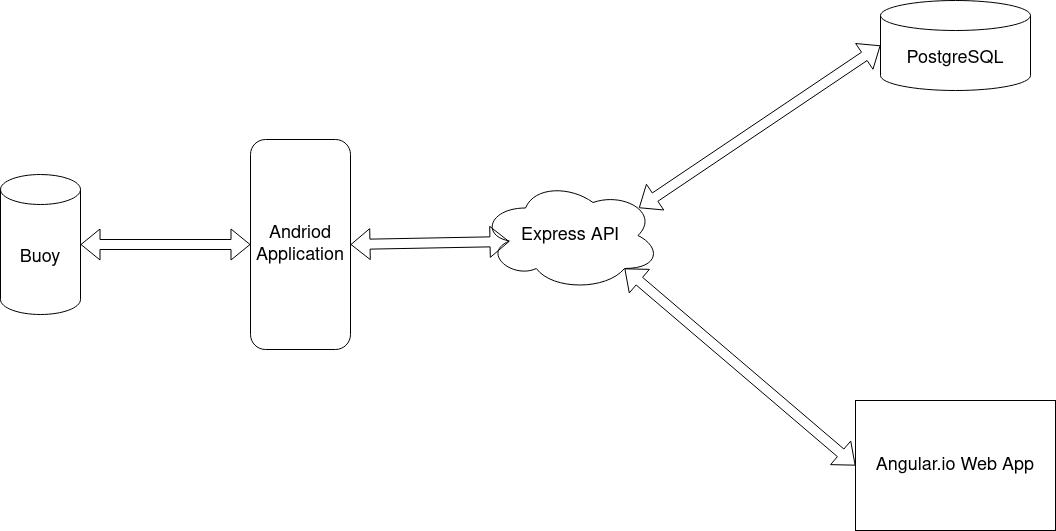
\includegraphics[scale=0.3]{wwxs.png}
\subsection{Web API Communication Protocol}
The goal of these API calls is to create, read, update and delete entries safley in the database. And to clearly communicate with the client (usually the web UI or the Mobile Application) the API must give meaningful responses. Any form of response designed to not return data will reply with JSON data with a message field. For example, a 200 "OK" response would return with this message in the body:
\begin{lstlisting}
  {
    message: "OK"
  }
\end{lstlisting}
In general, here are a list of create, read, update and delete calls and what they should return:
\begin{center}
  \begin{tabular}{| p{0.2\linewidth} | p{0.4\linewidth}  | p{0.4\linewidth} |}
    \hline
    HTTP Request Type & On success & On failure \\
    \hline
    GET "/" & 200 and all entries in the table & 400 Bad Request \\
    \hline
    GET "/:id" & 200 all entries in the table & 400 Bad Request \\
    & whose private key matches & 404 Not Found \\
    \hline
    POST "/" & 201 and the entry placed in the table & 400 Bad Request \\
    \hline
    PUT "/:id" & 200 and the entire entry updated & 400 Bad Request \\
    & with updated information & 404 Not Found \\
    \hline
    DELETE "/:id" & 200 OK & 400 Bad Request \\
    & & 404 Not Found \\
    \hline
  \end{tabular}
\end{center}
And the routes:
\begin{center}
  \begin{tabular}{| p{0.2\linewidth} | p{0.4\linewidth}  | p{0.4\linewidth} |}
    \hline
    Route & Description & Supported Methods \\
    \hline
    /buoy & Information associated with every buoy. & GET, GET + /:id, POST, PUT, DELETE + /:id \\
    \hline
    /data & Information associated with data pointed collected by buoys. & GET, GET + /:id, POST \\
    \hline
    /group & Information associated with groups of users. & GET, GET + /:id, POST, PUT, DELETE + /:id \\
    \hline
    /session & \emph{Deprecated} Information associated with user sessions. & \emph{Deprecated} \\
    \hline
    /user & Information associated with users and login. & GET, GET + /:id, POST \\
    \hline
    /user/login & Returns web token for authorization. & POST \\
    \hline
  \end{tabular}
\end{center}
\subsubsection{Buoy}
\texttt{
\{ \\
    "id": identification number (int)\\
    "name": meaningful buoy name (string)\\
    "mac": mac/hardware address of buoy (string)\\
    "pubKey": public key to encrypt information for buoy (string)\\
    "lastRetrieval": last date the buoy submitted data (sql date)\\
    "version": version of buoy (string)\\
    "createdAt": creation date (sql date)\\
    "updatedAt": updated date (sql date)\\
    "groupId": identification number the group the buoy belongs too (integer, foriegn key)\\
\}
}
\subsubsection{Data}
\texttt{
\{ \\
    "id": identification number (int) \\
    "updatedAt": updated date (sql date) \\
    "createdAt": creation date (sql date) \\
    "timestamp": collection timestamp (sql date) \\
    "surfTemp": surface temprature collected within the buoy (float) \\
    "surfInsolation": measure of sunlight exposure in the buoy (float) \\
    "shallowSalinity": measure of salinity at 2' depth (float) \\
    "shallowTemp": measure of water temprature at 2' depth (float) \\
    "depthTemp": measure of water temprature at 7' depth (float) \\
    "depthTurbidity": measure of sunlight at 7' depth (float) \\
    "buoyId": id of buoy that collected the data (int, foreign key) \\
    "userId": id of user that collected the data (int, foreign key) \\
\}
}
\subsubsection{Group}
\texttt{
\{ \\
    "id": identification number (int) \\
    "name": meaningful group name (string) \\
    "updatedAt": updated date (sql date) \\
    "createdAt": creation date (sql date) \\
\}
}
\subsubsection{User}
\texttt{
\{ \\
    "id": identification number (int) \\
    "updatedAt": updated date (sql date) \\
    "createdAt": creation date (sql date) \\
    "username": meaningful username (string) \\
    "password": meaninful password (string) \\
    "email": user's email (string) \\
    "role":  user's role (string) \\
    "lastLogin": last login date (sql date) \\
    "groupId": identification number the group the user belongs to (integer, foriegn key) \\
    "token": string formatted JSON web token (string) \\
\}
}
% make a 1;1 list of every route and method in the node.js api
